\section{Ablaufdiagramme}

\subsection{Import von Daten}

Dieses Sequenzdiagramm beschreibt den Verlauf des Imports von Daten vom "{Upload}"{-Button} aus.
Dazu wird vom MainWindow erst der Import-Controller aufgerufen.
Dort wird mit den Informationen von der Weboberfläche eine Konfiguration erstellt und damit zusammen mit dem Namen der Quelldatei der UploadHandler aufgerufen.
Dieser lädt erst die Quelldatei und konvertiert die Daten aus der Quelldatei in die interne RowTable-Darstellung.
Anschließend wird diese in eine ColumnTable umgewandelt um dann spaltenweise mit convertTable() die Datentypen der Daten anzupassen.
Danach wird wieder eine RowTable erstellt und diese zeilenweise abgearbeitet (siehe \ref{verarbeitung}).
\vspace{\fill}
\begin{figure}[htbp]
\centering
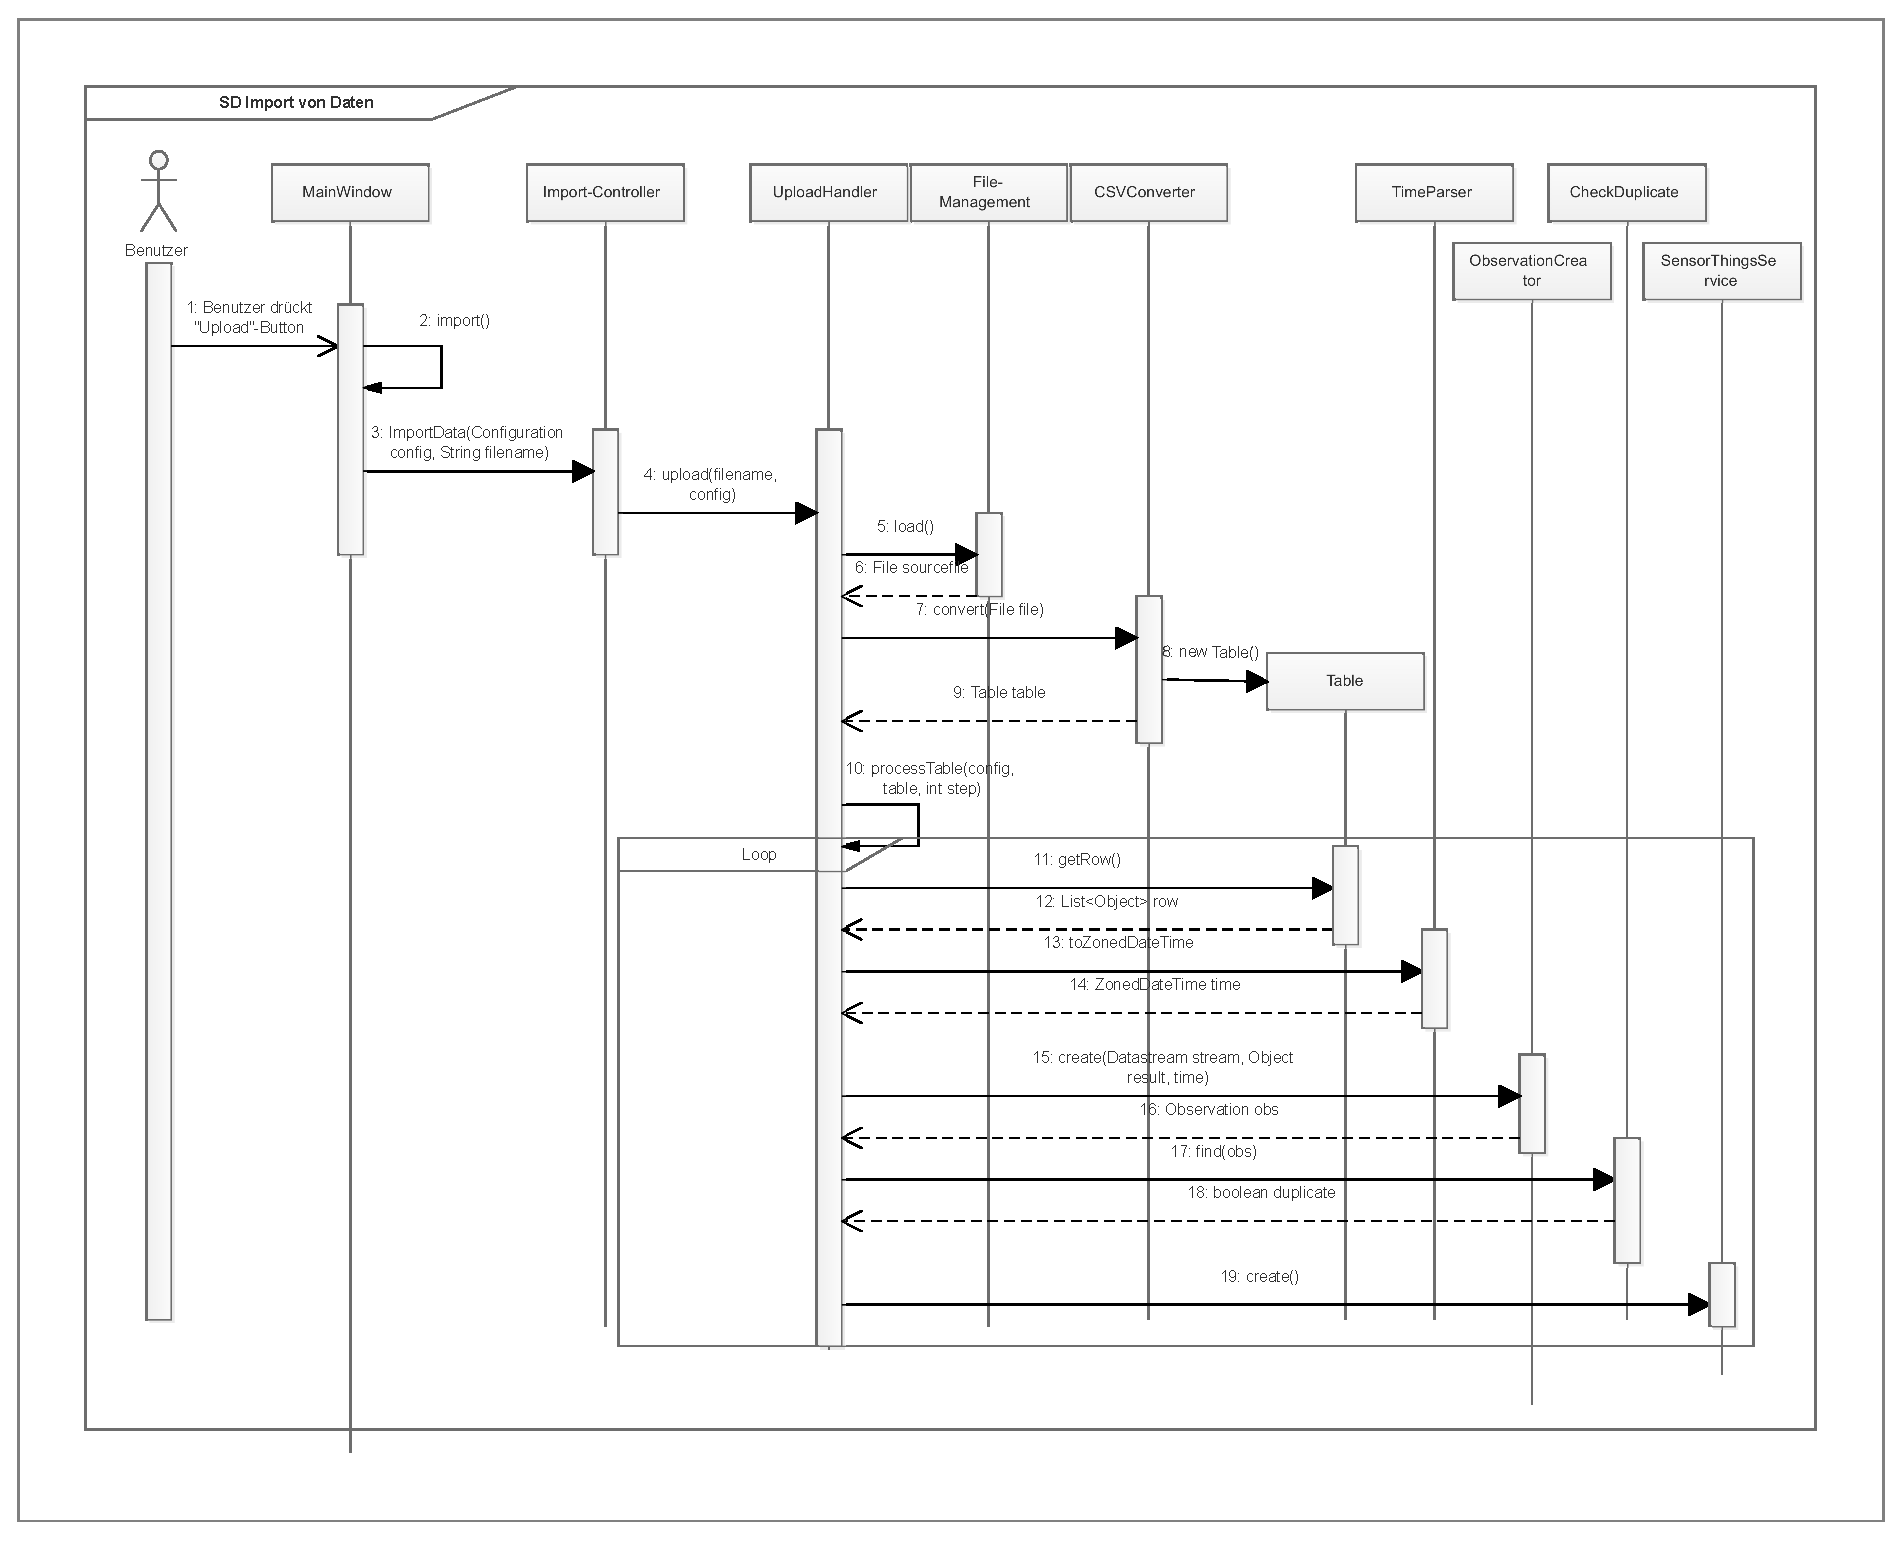
\includegraphics[scale=0.45]{uml/SD_upload.eps}
\caption{Sequenzdiagramm zum Import von Daten auf den FROST-Server}
\end{figure}
\vspace{\fill}

\subsubsection{Zeilenverarbeitung}\label{verarbeitung}

Das Sequenzdiagramm stellt die zeilenweise Verarbeitung der Daten aus der internen Darstellung zu Observations durch evaluateRow() dar.
Dazu werden mithilfe der Konfiguration die Zeilen für das Datumsformat ausgelesen und über den TimeParser in eine ZonedDateTime konvertiert.
Anschließend wird für diese Zeit und das Result aus der Zeile mit der CheckDuplicate-Klasse der FROST-Server auf Duplikate überprüft.
Gibt es keins, wird eine neue Observation mit dem Result und der Zeit erstellt und über den SensorThingsService auf dem FROST-Server erstellt.

\vspace{\fill}
\begin{figure}[htbp]
\centering
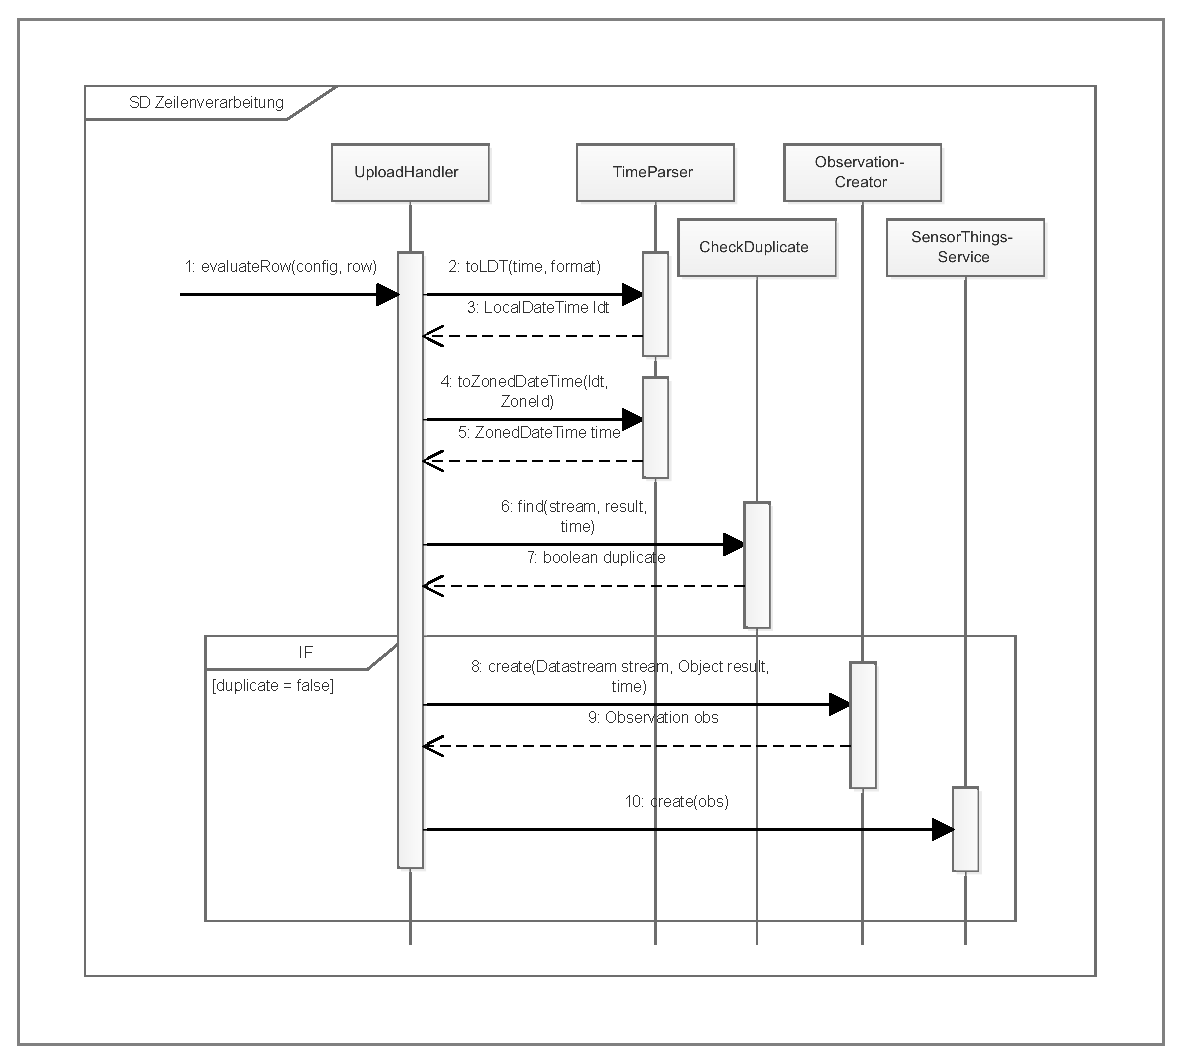
\includegraphics[scale=0.6]{uml/SD_row.eps}
\caption{Sequenzdiagramm für die Verarbeitung einer Zeile aus der internen Darstellung zu einer Observation}
\end{figure}
\vspace{\fill}

\clearpage
\subsection{Konfiguration speichern}
Das folgende Sequenzdiagramm beschreibt den Ablauf für das Speichern einer Konfiguration.
Drückt der Nutzer auf den ”{Save Configuration}"{-Button}, ruft das MainWindow den Konfigurations-Controller auf.
Dort wird mit den Eingabe-Daten von der Webseite eine Konfiguration erstellt und an das Config-Management zum Abspeichern übergeben.
Dieses konvertiert die Konfiguration erst in einen String, um diesen dann in einer Datei abzuspeichern.
\vspace{\fill}
\begin{figure}[htbp]
\centering
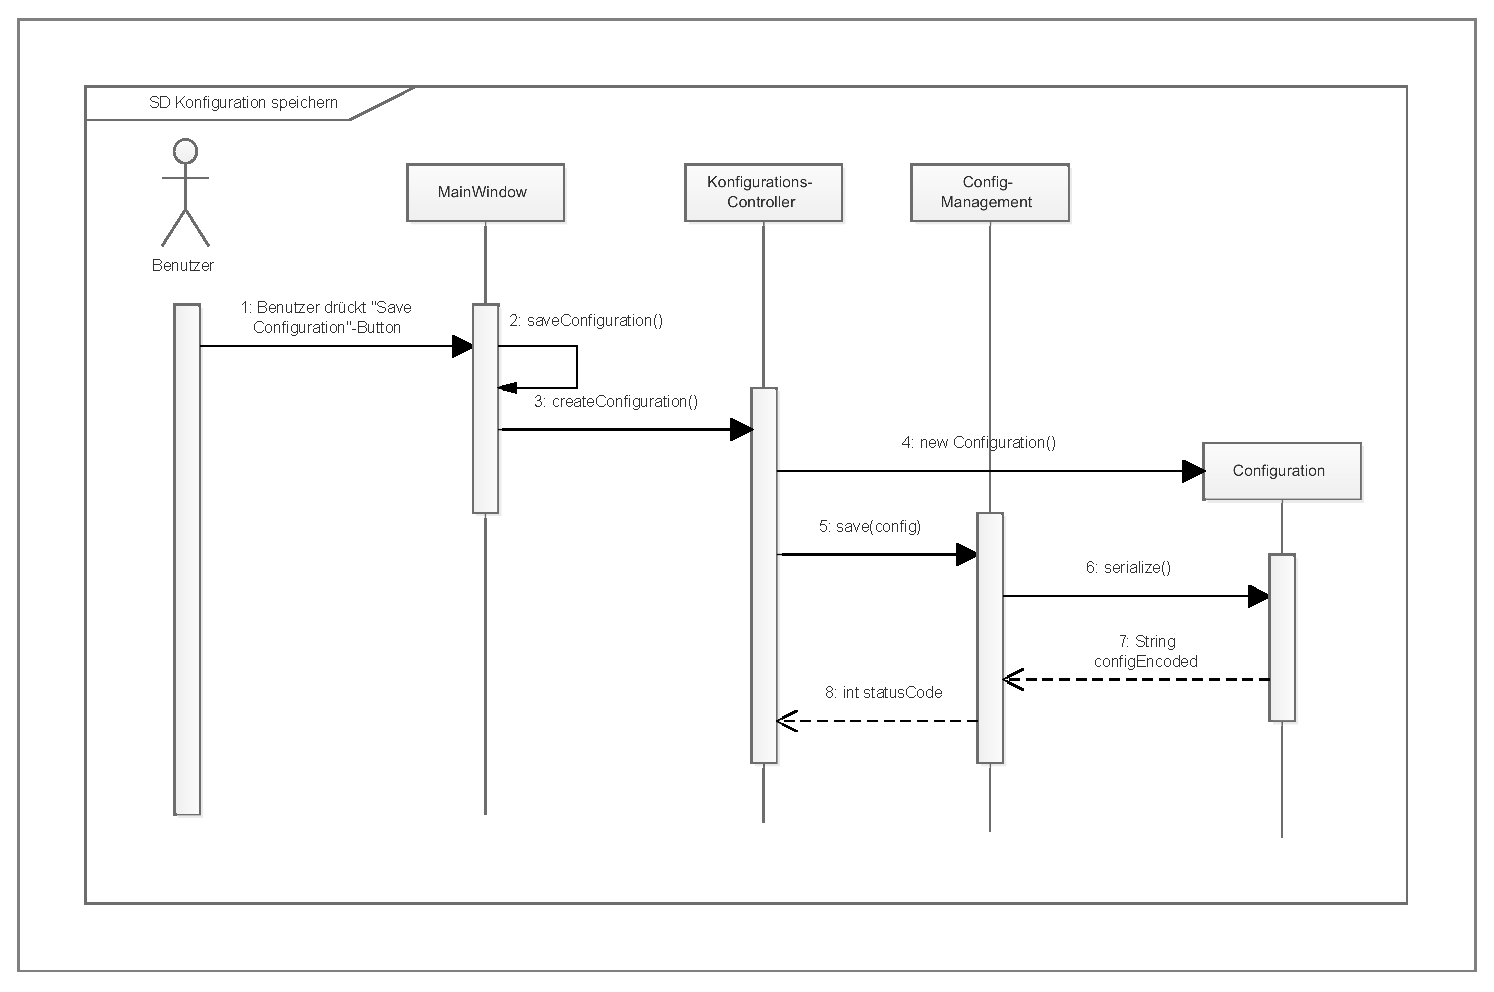
\includegraphics[scale=0.5]{uml/SD_saveConfig.eps}
\caption{Sequenzdiagramm zum Speichern einer Konfiguration}
\end{figure}

\vspace{\fill}
\clearpage
\subsection{Fehlerhafte Zeilen zurückgeben}
Das folgende Sequenzdiagramm beschreibt, was geschieht, wenn aus den Daten einer Zeile keine Observation erstellt werden kann.
Dazu wird dem ErrorHandler die Nummer der fehlerhaften Zeile und die geworfene Exception übergeben.
Nachdem alle Zeilen abgearbeitet wurden, wird dann die returnRows()-Methode im ErrorHandler aufgerufen.
Dort wird eine RowTable mit den fehlerhaften Zeilen erstellt.
Diese wird in eine Datei umgeschrieben und dann dem Nutzer über die donloadError-Funktion im MainWindow zur Rückgabe angeboten.

\vspace{\fill}
\begin{figure}[htbp]
\centering
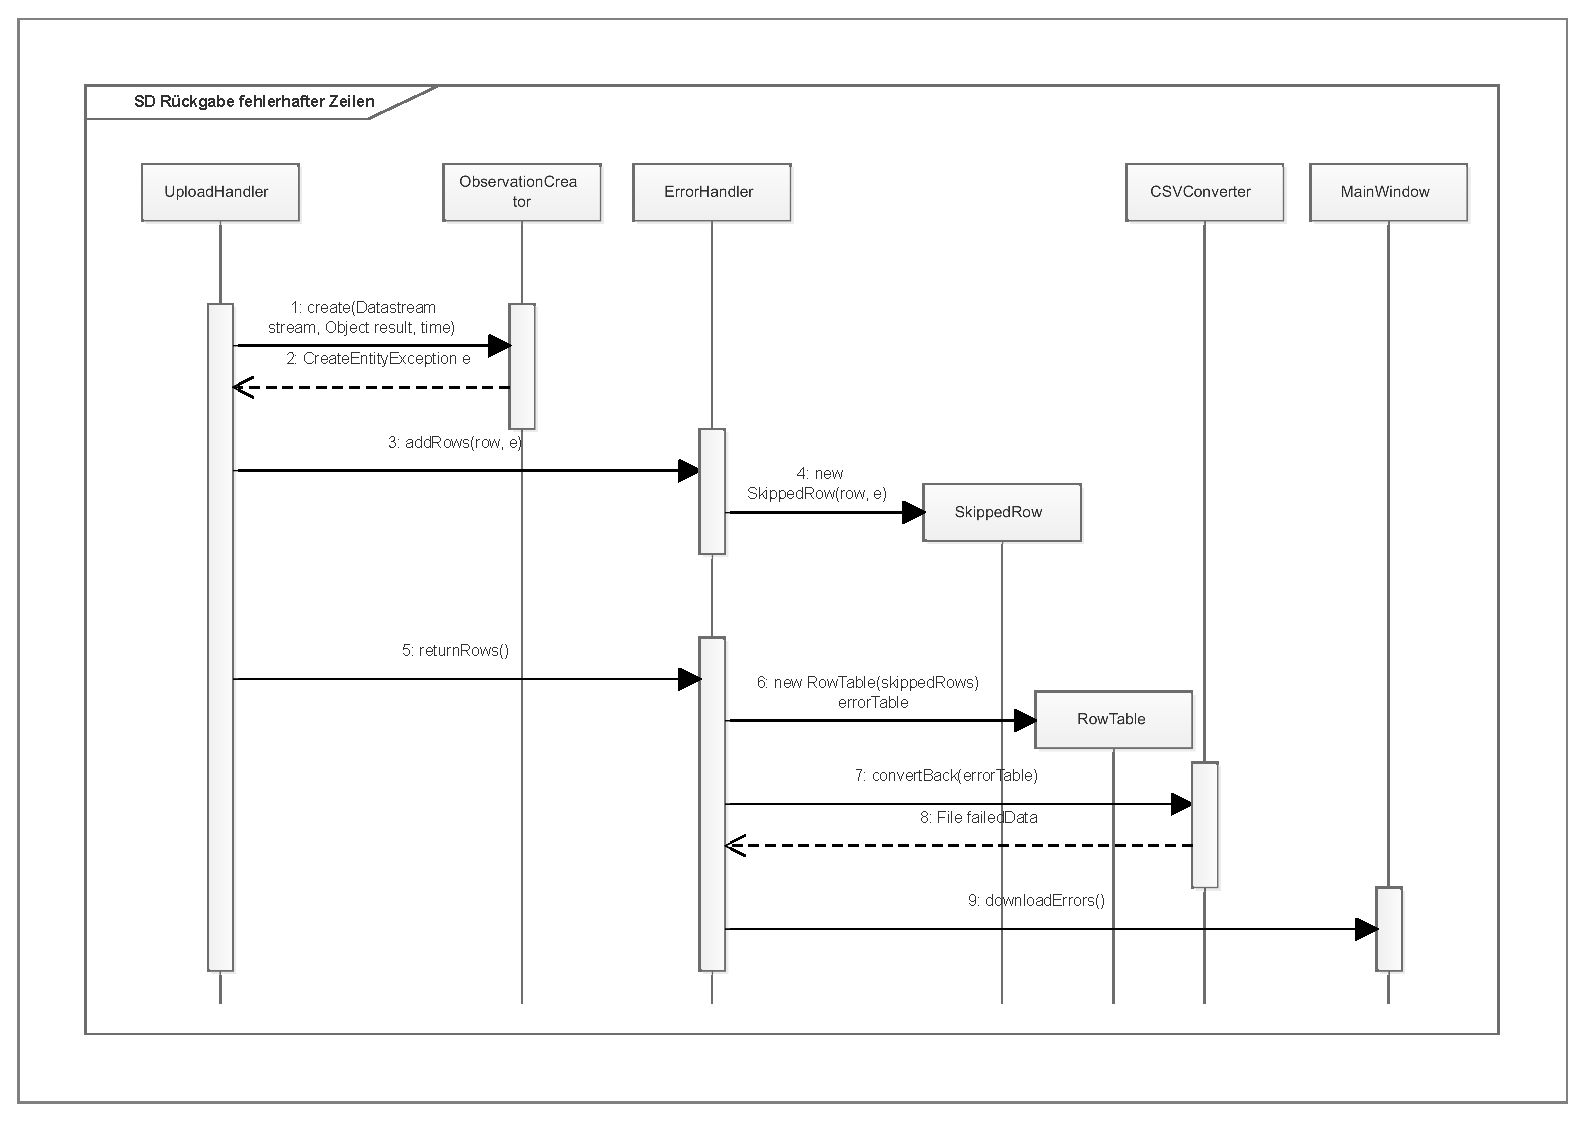
\includegraphics[scale=0.5]{uml/SD_returnErrors.eps}
\caption{Sequenzdiagramm zur Rückgabe fehlerhafter Zeilen als Datei}
\end{figure}
\vspace{\fill}

\clearpage
\subsection{Thing erstellen}

Im Sequenzdiagramm wird dargestellt, was beim Erstellen eines Things passiert.
Das Erstellen anderer Entities verläuft analog.
Beim Klicken auf den "{Create Thing}"{-Button} reagiert das MainWindow und öffnet einen Dialog zum Erstellen des Things.
Dort lassen sich die Eigenschaften des Things vom Benutzer festlegen.
Beim Auswahl der Location werden die Vorschläge über die Funktion chooseLocation() aktualisiert.
Dazu wird über den LocationController eine Anfrage an den SensorThingsService gestellt, um alle bestehenden Locations abzufragen.
Die bestehenden Locations werden im Body einer ResponseEntity an das ThingWindow zurückgegeben.
Mit diesen werden dem Benutzer Vorschläge für eine Location angezeigt.
Nach dem der Benutzer eine Location gewählt und den den "{Create}"{-Button} gedrückt hat, wird der ThingController aufgerufen, um das Thing zu erstellen.
Dazu ruft er erneut den SensorThingsService auf und gibt nach Ausführung der Operation eine ResponseEntity zurück, um das Ergebnis der Operation zu beschreiben.
Abschließend wird das ThingWindow geschlossen und dem Nutzer wieder das MainWindow angezeigt.

\vspace{\fill}

\begin{figure}[htbp]
\centering
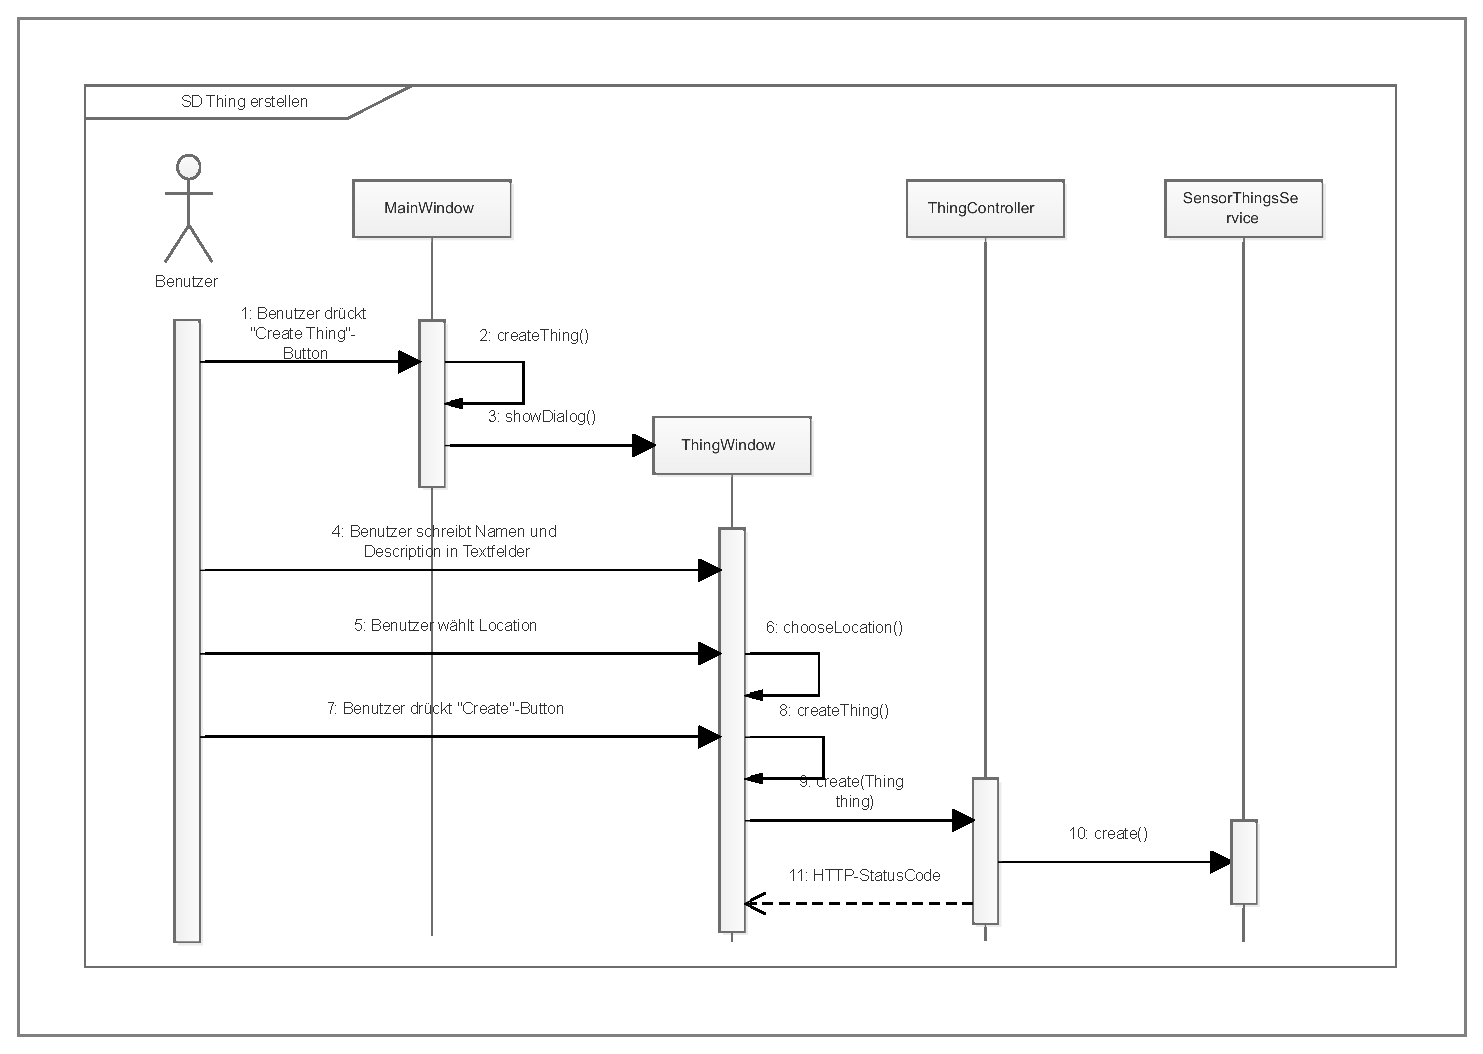
\includegraphics[scale=0.52]{uml/SD_createThing.eps}
\caption{Sequenzdiagramm zum Erstellen eines Things auf dem FROST-Server}
\end{figure}

\vspace{\fill}
\clearpage
\subsection{Quelldatei wählen}
Dieses Sequenzdiagramm zeigt den Ablauf für die Auswahl einer Quelldatei durch den Nutzer.
Drückt der Nutzer den "{Browse}"{-Button}, wird der SourceFileController mit der ausgewählten Quelldatei aufgerufen.
Diese wird dann dem FileManager zum Abspeichern übergeben.
Abschließend wird dem Nutzer eine Meldung mit dem Ergebnis der Operation angezeigt.

\vspace{\fill}
\begin{figure}[htbp]
\centering
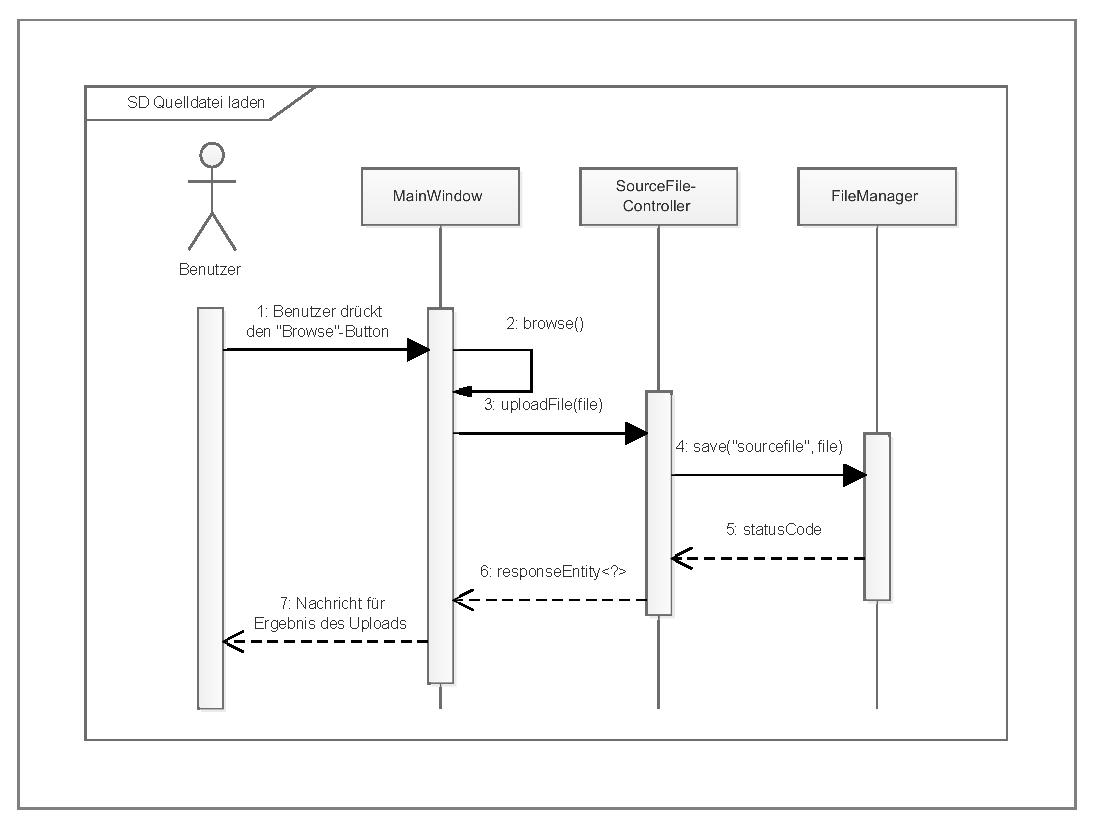
\includegraphics[scale=0.7]{uml/SD_sourceFile.eps}
\caption{Sequenzdiagramm zum Auswählen einer Quelldatei}
\end{figure}

\vspace{\fill}